\documentclass{report}
\usepackage{fullpage}
\usepackage{titlesec}
\usepackage{booktabs}
\titleformat{\chapter}[display]
  {\normalfont\bfseries}{}{0pt}{\Huge}
\renewcommand{\baselinestretch}{1}
\usepackage{float}
\usepackage{subfig}
\usepackage{graphicx}

\usepackage{geometry}
 \geometry{
 a4paper,
 total={170mm,257mm},
 left=20mm,
 top=20mm,
 }

\begin{document}

\chapter{Comparing Results}

In this report, Machine Learning results are compared when we include redshift dependant features amoung the features we obtained from busy function fitting and excluding the redshift dependant features. As usual we have Random Forest, Decision tree, KNN, Logistic Regression and SVM as machine Learning Models. Normal Neural network has failed in both the cases as it requires a large amount of data to train, but CNN showed it can be trained, as it has been overfitting using previous data. We can train CNN by cropping the spectra and feeding it. But how the spectra should be cropped has been an issue as the widths are uneven between Associated and Intervening spectra. During the meetings with Dr Banerjee, we have decided to crop just the spectra i.e only the part where spectra is seen. This work is kind of troublesome, but I can get it done.

Here, we compare ROC AUC, Accuracy and Precision. Just to recap, ROC AUC is the area under the reciever operating characteristic curve. This ROC AUC can be interpreted as the proability that the model predicts a random positive sample more highly than a random negative sample. It should be near 1 to make sure the model is predicted correctly. Average Accuracy and Average precision talks about the accuracy and precision of the model.

\section{Comapring ROC AUC, Accuracy and Precision}
\subsection{When Redshift dependant features are added}
\begin{table}[h] 
  \centering
  \begin{tabular}{@{}cc@{}cc@{}cc@{}}
    \toprule
    ML Model & ROC AUC  | & Average Accuracy & Average Precision  \\
    \midrule
    Random Forest & $0.942$ & $88.9\%$ & $92.6\%$ \\
    KNN & $0.882$ & $82.1\%$ & $85.1\%$ \\
    Decision Tree & $0.754$ & $75.5\%$ & $67.2\%$ \\
    Logistic Regression & $0.854$ & $76.9\%$ & $82.7\%$ \\
    SVM & $0.842$ & $76.6\%$ & $82.4\%$ \\
    \bottomrule
  \end{tabular}
  \caption{Results for Machine Learning models incluing redshift dependant features.}
  \label{results_1}
\end{table}

\subsection{When Redshift dependant features are not added}
\begin{table}[h] 
  \centering
  \begin{tabular}{@{}cc@{}cc@{}cc@{}}
    \toprule
    ML Model & ROC AUC  | & Average Accuracy & Average Precision  \\
    \midrule
    Random Forest & $ 0.864$ & $79.9\%$ & $82.5\%$ \\
    KNN & $0.775$ & $71.4\%$ & $76.8\%$ \\
    Decision Tree & $0.812$ & $81.6\%$ & $74.9\%$ \\
    Logistic Regression & $0.510$ & $46.5\%$ & $62.2\%$ \\
    SVM & $0.557$ & $48.9\%$ & $63.2\%$ \\
    \bottomrule
  \end{tabular}
  \caption{Results for Machine Learning models not incluing redshift dependant features.}
  \label{results_2}
\end{table}

\newpage
\section{Comparing the ROC Curves}
\subsection{When Redshift dependant features are added}

\begin{figure}[H]%
    \centering
    \subfloat[\centering Random Forest]{{\includegraphics[width=7.5cm]{ROC_curve_random_forest_smote_r.png} }}%
    \qquad
    \subfloat[\centering KNN]{{\includegraphics[width=7.5cm]{ROC_curve_knn_smote_r.png} }}%
    \qquad
    \subfloat[\centering Decision Tree]{{\includegraphics[width=7.5cm]{ROC_curve_decision_tree_smote_r.png} }}%
    \qquad
    \subfloat[\centering Logistic Regression]{{\includegraphics[width=7.5cm]{ROC_curve_logistic_regression_smote_r.png} }}%
    \qquad
    \subfloat[\centering SVM]{{\includegraphics[width=7.5cm]{ROC_curve_SVM_smote_r.png} }}%
    \caption{Mean ROC curve plots for all models when redhsift dependant features are added}%
    \label{fig:1}%
\end{figure}
\subsection{When Redshift dependant features are not added}

\begin{figure}[H]%
    \centering
    \subfloat[\centering Random Forest]{{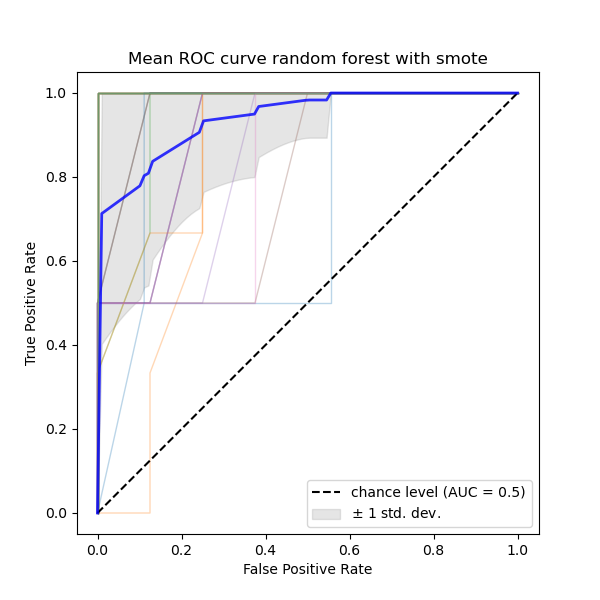
\includegraphics[width=7.5cm]{ROC_curve_random_forest_smote.png} }}%
    \qquad
    \subfloat[\centering KNN]{{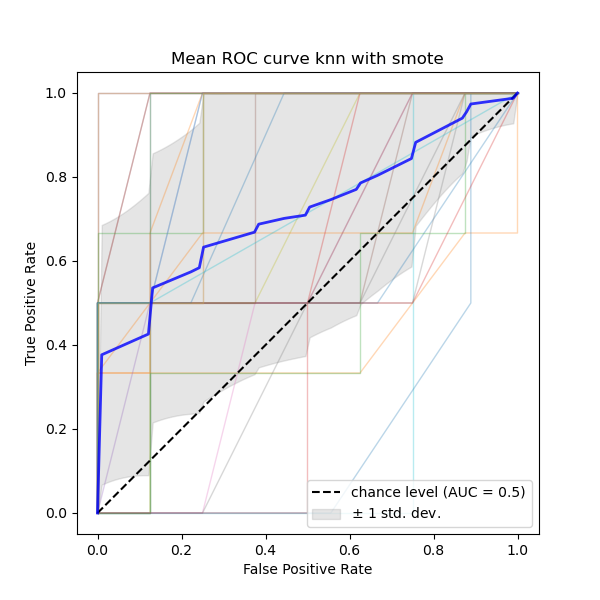
\includegraphics[width=7.5cm]{ROC_curve_knn_smote.png} }}%
    \qquad
    \subfloat[\centering Decision Tree]{{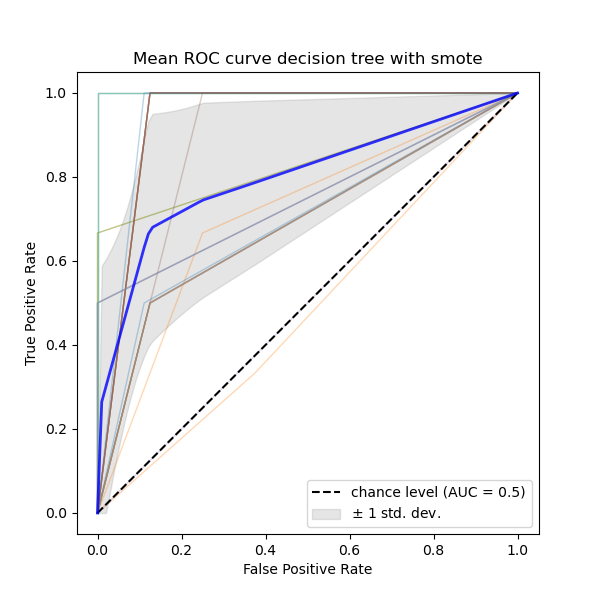
\includegraphics[width=7.5cm]{ROC_curve_decision_tree_smote.png} }}%
    \qquad
    \subfloat[\centering Logistic Regression]{{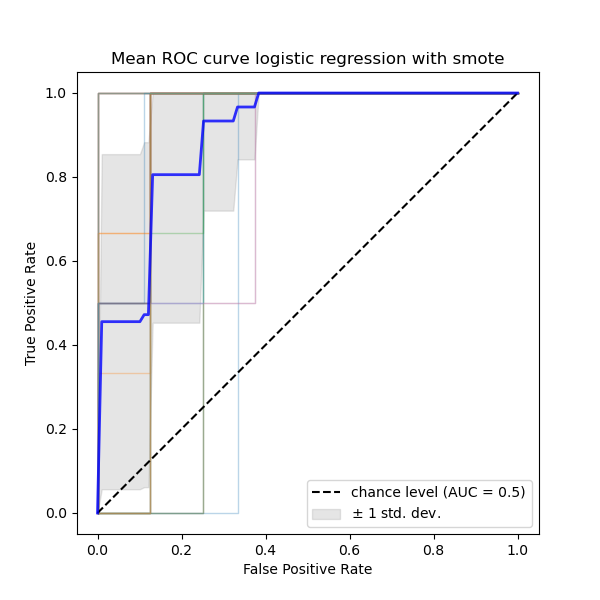
\includegraphics[width=7.5cm]{ROC_curve_logistic_regression_smote.png} }}%
    \qquad
    \subfloat[\centering SVM]{{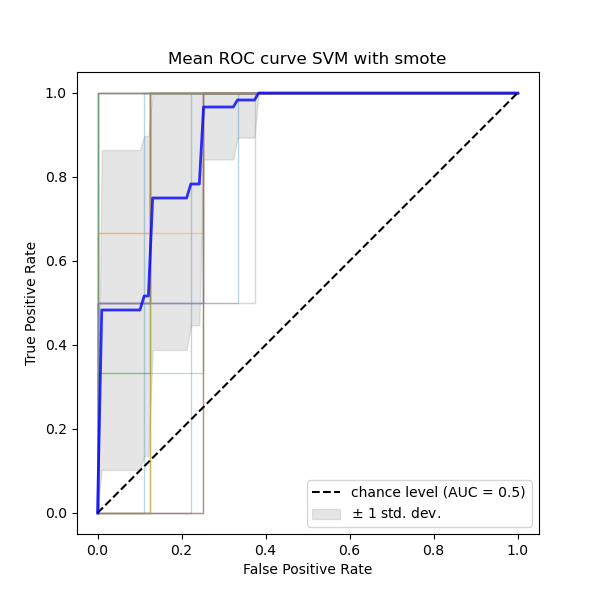
\includegraphics[width=7.5cm]{ROC_curve_SVM_smote.png} }}%
    \caption{Mean ROC curve plots for all models when redhsift dependant features are not added}%
    \label{fig:2}%
\end{figure}

\end{document}